\documentclass[12pt, a4paper, oneside]{ctexart}
\usepackage{amsmath, amsthm, amssymb, bm, color, framed, graphicx, hyperref, mathrsfs, float, caption,subfigure}
\usepackage[justification=centering]{caption}

% multi-column
\usepackage{tasks}
% itemize
\NewTasksEnvironment[label=(\arabic*), label-width=3ex]{exercise}

\everymath{\displaystyle}

\title{\textbf{第六次作业}}
\author{U08M11002 Fall 2023}
\linespread{1}
\definecolor{shadecolor}{RGB}{241, 241, 255}

\newcounter{problemname}
\newenvironment{problem}{\stepcounter{problemname}\par\noindent\textbf{题目\arabic{problemname}. }}{\\\par}
\newenvironment{warning}{\begin{shaded}\par\noindent\textbf{提交作业方式:}}{\end{shaded}\par}


\begin{document}
	
	\maketitle
	
	\hspace{1em}
	
	
	\begin{problem}
		求下列各像函数$F(S)$的原函数$f(t)$。
		\begin{exercise}
			\task $F(s) = \frac{s^3 + 6s^2 +6s}{s^2 + 6s +8}$;
			\task $F(s) = \frac{1}{s^2(s + 1)^3}$;
			\task $F(s) = \frac{2 + e^{-(s - 1)}}{(s - 1)^2 + 4}$;
			\task $F(s) = \frac{1}{s(1 - e^{-s})}$;
			\task 	$F(s) = \left(\frac{1 - e^{-s}}{s}\right) ^{2}$;
		\end{exercise}
	
		\quad
	\end{problem}
	
	\begin{problem}
		判断下列叙述是否正确:
		\begin{exercise}
			\task 一个信号存在拉普拉斯变换,就一定存在傅里叶变换。
			\task 一个信号存在傅里叶变换,就一定存在单边拉普拉斯变换。
			\task 一个信号存在傅里叶变换,就一定存在双边拉普拉斯变换。
	\end{exercise}
		\quad
	\end{problem}
	
	\begin{problem}
		连续系统的微分方程为$y^{''}(t) + 4y^{'}(t) + 4y(t) = f^{'}(t) + 3f(t)$,当激励$f(t) = e^{-t}U(t)$时,其全响应的初始值$y(0^{+}) = 1$,$y^{'}(0^{+}) = 3$。求系统的全响应$y(t)$,零状态响应$y_f(t)$,零输入响应$y_x(t)$。
		\quad
	\end{problem}
	
	\newpage 
	\begin{problem}
	已知系统函数$H(s)$的零极点分布如图1所示,$h(0^{+}) = \sqrt{2}$。求$H(s)$及单位冲激响应$h(t)$。
		\begin{figure}[H]
			
\includegraphics[width=10cm]{assets/hw7img1.png}
			\centering
			\caption{}
		\end{figure}
		
		\quad
	\end{problem}
	
	
	\newpage
	\begin{problem}
		已知系统函数$H(s)$的零极点分布如图2所示,$h(0^{+}) = 1$,激励$f(t) = \cos(wt)U(t)$,分别对以下几种情况求零状态响应$y(t)$:
		\begin{exercise}
		  \task $w = 0$;
		  \task $w = 1 \mathrm{rad/s}$;
		  \task $w = 2 \mathrm{rad/s}$;
		\end{exercise}

		\begin{figure}[H]
			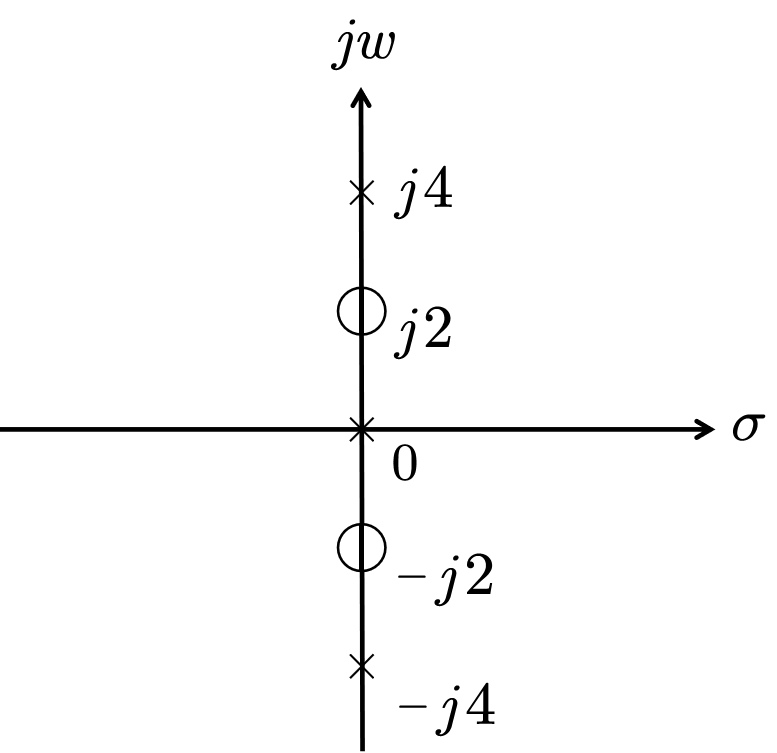
\includegraphics[width=10cm]{assets/hw7img2.png}
			\centering
			\caption{}
		\end{figure}
		\quad
	\end{problem}
	
	\newpage
	\begin{problem}
		已知线性时不变稳定系统$H(s)$的零极点分布如图3所示,系统的激励$f(t) = e^{3t}$,$t\in R$,响应$y(t) = \frac{3}{20}e^{3t}$,$t\in R$。
		(\textbf{注意:该题存在问题,找出并解释错误!})
		\begin{exercise}
			\task 求$H(s)$及$h(t)$,判断系统是否为因果系统;
			\task 若$f(t) = U(t)$,求响应$y(t)$;
			\task 求系统的微分方程;
			\task 画出系统的信号流图。
		\end{exercise}
	
		\begin{figure}[H]
			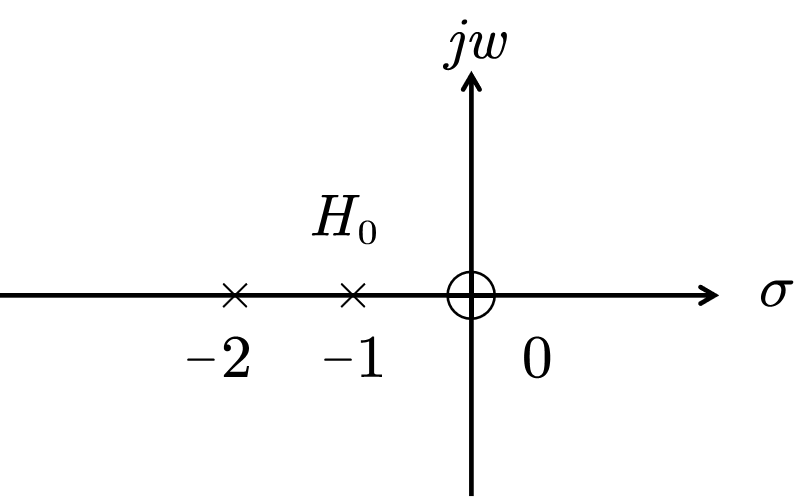
\includegraphics[width=10cm]{assets/hw7img3.png}
			\centering
			\caption{}
		\end{figure}
		\quad
	\end{problem}
	\newpage
	
	\begin{problem}
		图4所示为非零状态系统,已知激励$f(t) = U(t)$时的全响应$y(t) = (1 - e^{-t} + e^{-3t})U(t)$。
		\begin{exercise}
			\task 求常数$a$,$b$,$c$的值;
			\task 求零输入响应$y_x(t)$;
			\task 若$f(t) = 10\sqrt{5}\cos(3t - 63.4^{\circ})$,求稳态响应$y(t)$。
		\end{exercise}
		
		\begin{figure}[H]
			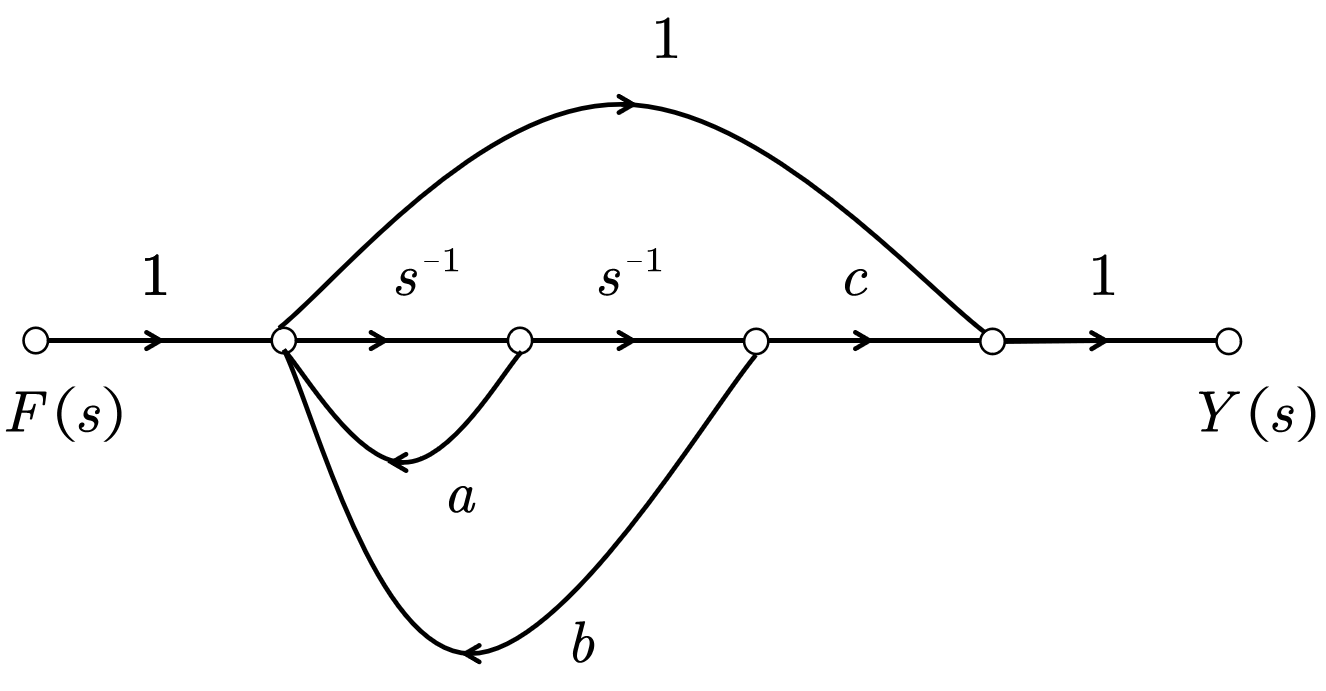
\includegraphics[width=10cm]{assets/hw7img4.png}
			\centering
			\caption{}
		\end{figure}
		\quad
	\end{problem}
	
	\begin{problem}
		已知连续系统的微分方程为$y^{''}(t) + 7y^{'}(t) + 10y(t) = 2f^{'}(t) + 3f(t)$,且有$f(t) = e^{-t}U(t)$,$y(0^{-}) = 1$,$y^{'}(0^{-}) = 1$。由$s$域求解:
		\begin{exercise}
			\task 零输入响应与零状态响应;
			\task 系统函数$H(s)$,单位冲激响应$h(t)$,判断系统是否稳定。
		\end{exercise}
	
		\quad
	\end{problem}
	\newpage
	\begin{problem}
		系统框图如图5所示。
		\begin{exercise}
			\task 画出其对应的模拟图与信号流图;
			\task 求$H(s) = \frac{Y(s)}{F(s)}$。
			
		\end{exercise}
		\begin{figure}[H]
			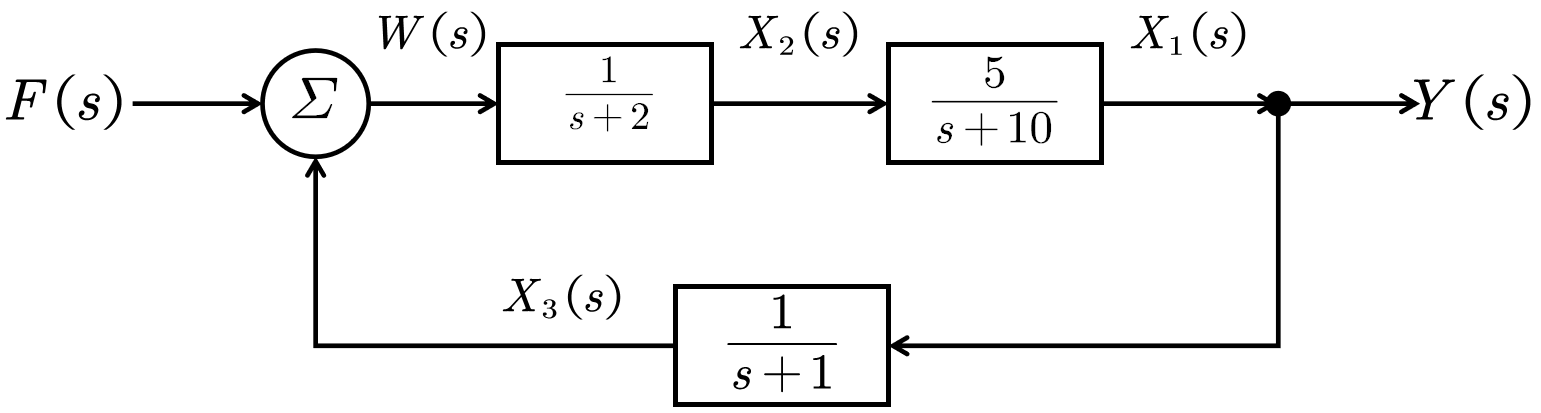
\includegraphics[width=15cm]{assets/hw7img5.png}
			\centering
			\caption{}
		\end{figure}
		\quad
	\end{problem}
	
	\begin{problem}
		求下列函数的单边拉普拉斯变换,并注明收敛域。
		\begin{exercise}
			\task $1 - e^{-t}$;
			\task $1-2e^{-t} + e^{-2t}$;
			\task $3\sin t + 2\cos t$;
			\task $\cos(2t + 45^{\circ})$;
			\task $e^{t} + e^{-t}$;
			\task $e^{-t}\sin(2t)$;
			\task $te^{-2t}$;
			\task $2\delta(t) - e^{-t}$;
			
		\end{exercise}
		\quad
	\end{problem}	
	
	\newpage
	\begin{problem}
		描述某LTI系统的微分方程$y^{'}(t) + 2y(t) = f^{'}(t) + f(t)$,求在下列激励下的零状态响应。
		\begin{exercise}
			\task $f(t) = U(t)$;
			\task $f(t) = e^{-t}U(t)$;
			\task $f(t) = e^{-2t}U(t)$;
			\task $f(t) = tU(t)$;
		\end{exercise}
		\quad
	\end{problem}
	
	\begin{problem}
		描述某$\mathrm{LTI}$系统的微分方程为:$y^{''}(t) + 3y^{'}(t) + 2y(t) = f^{'}(t) + 4f(t)$,求在下列条件下的零输入响应和零状态响应:
		\begin{exercise}
			\task $f(t) = U(t)$,$y(0_{-}) = 0$,$y^{'}(0_{-}) = 1$
			\task $f(t) = e^{-2t}U(t)$,$y(0_{-}) = 1$,$y^{'}(0_{-}) = 1$
		\end{exercise}
	\quad
	\end{problem}
	
\end{document}